\subsection{UML Description}

\textbf{Use Case Diagram} \\
The figure below shows the Use Case diagram of CLup, which summarises use cases and the actors who perform them. \\
\begin{figure}[H] 
\centerline{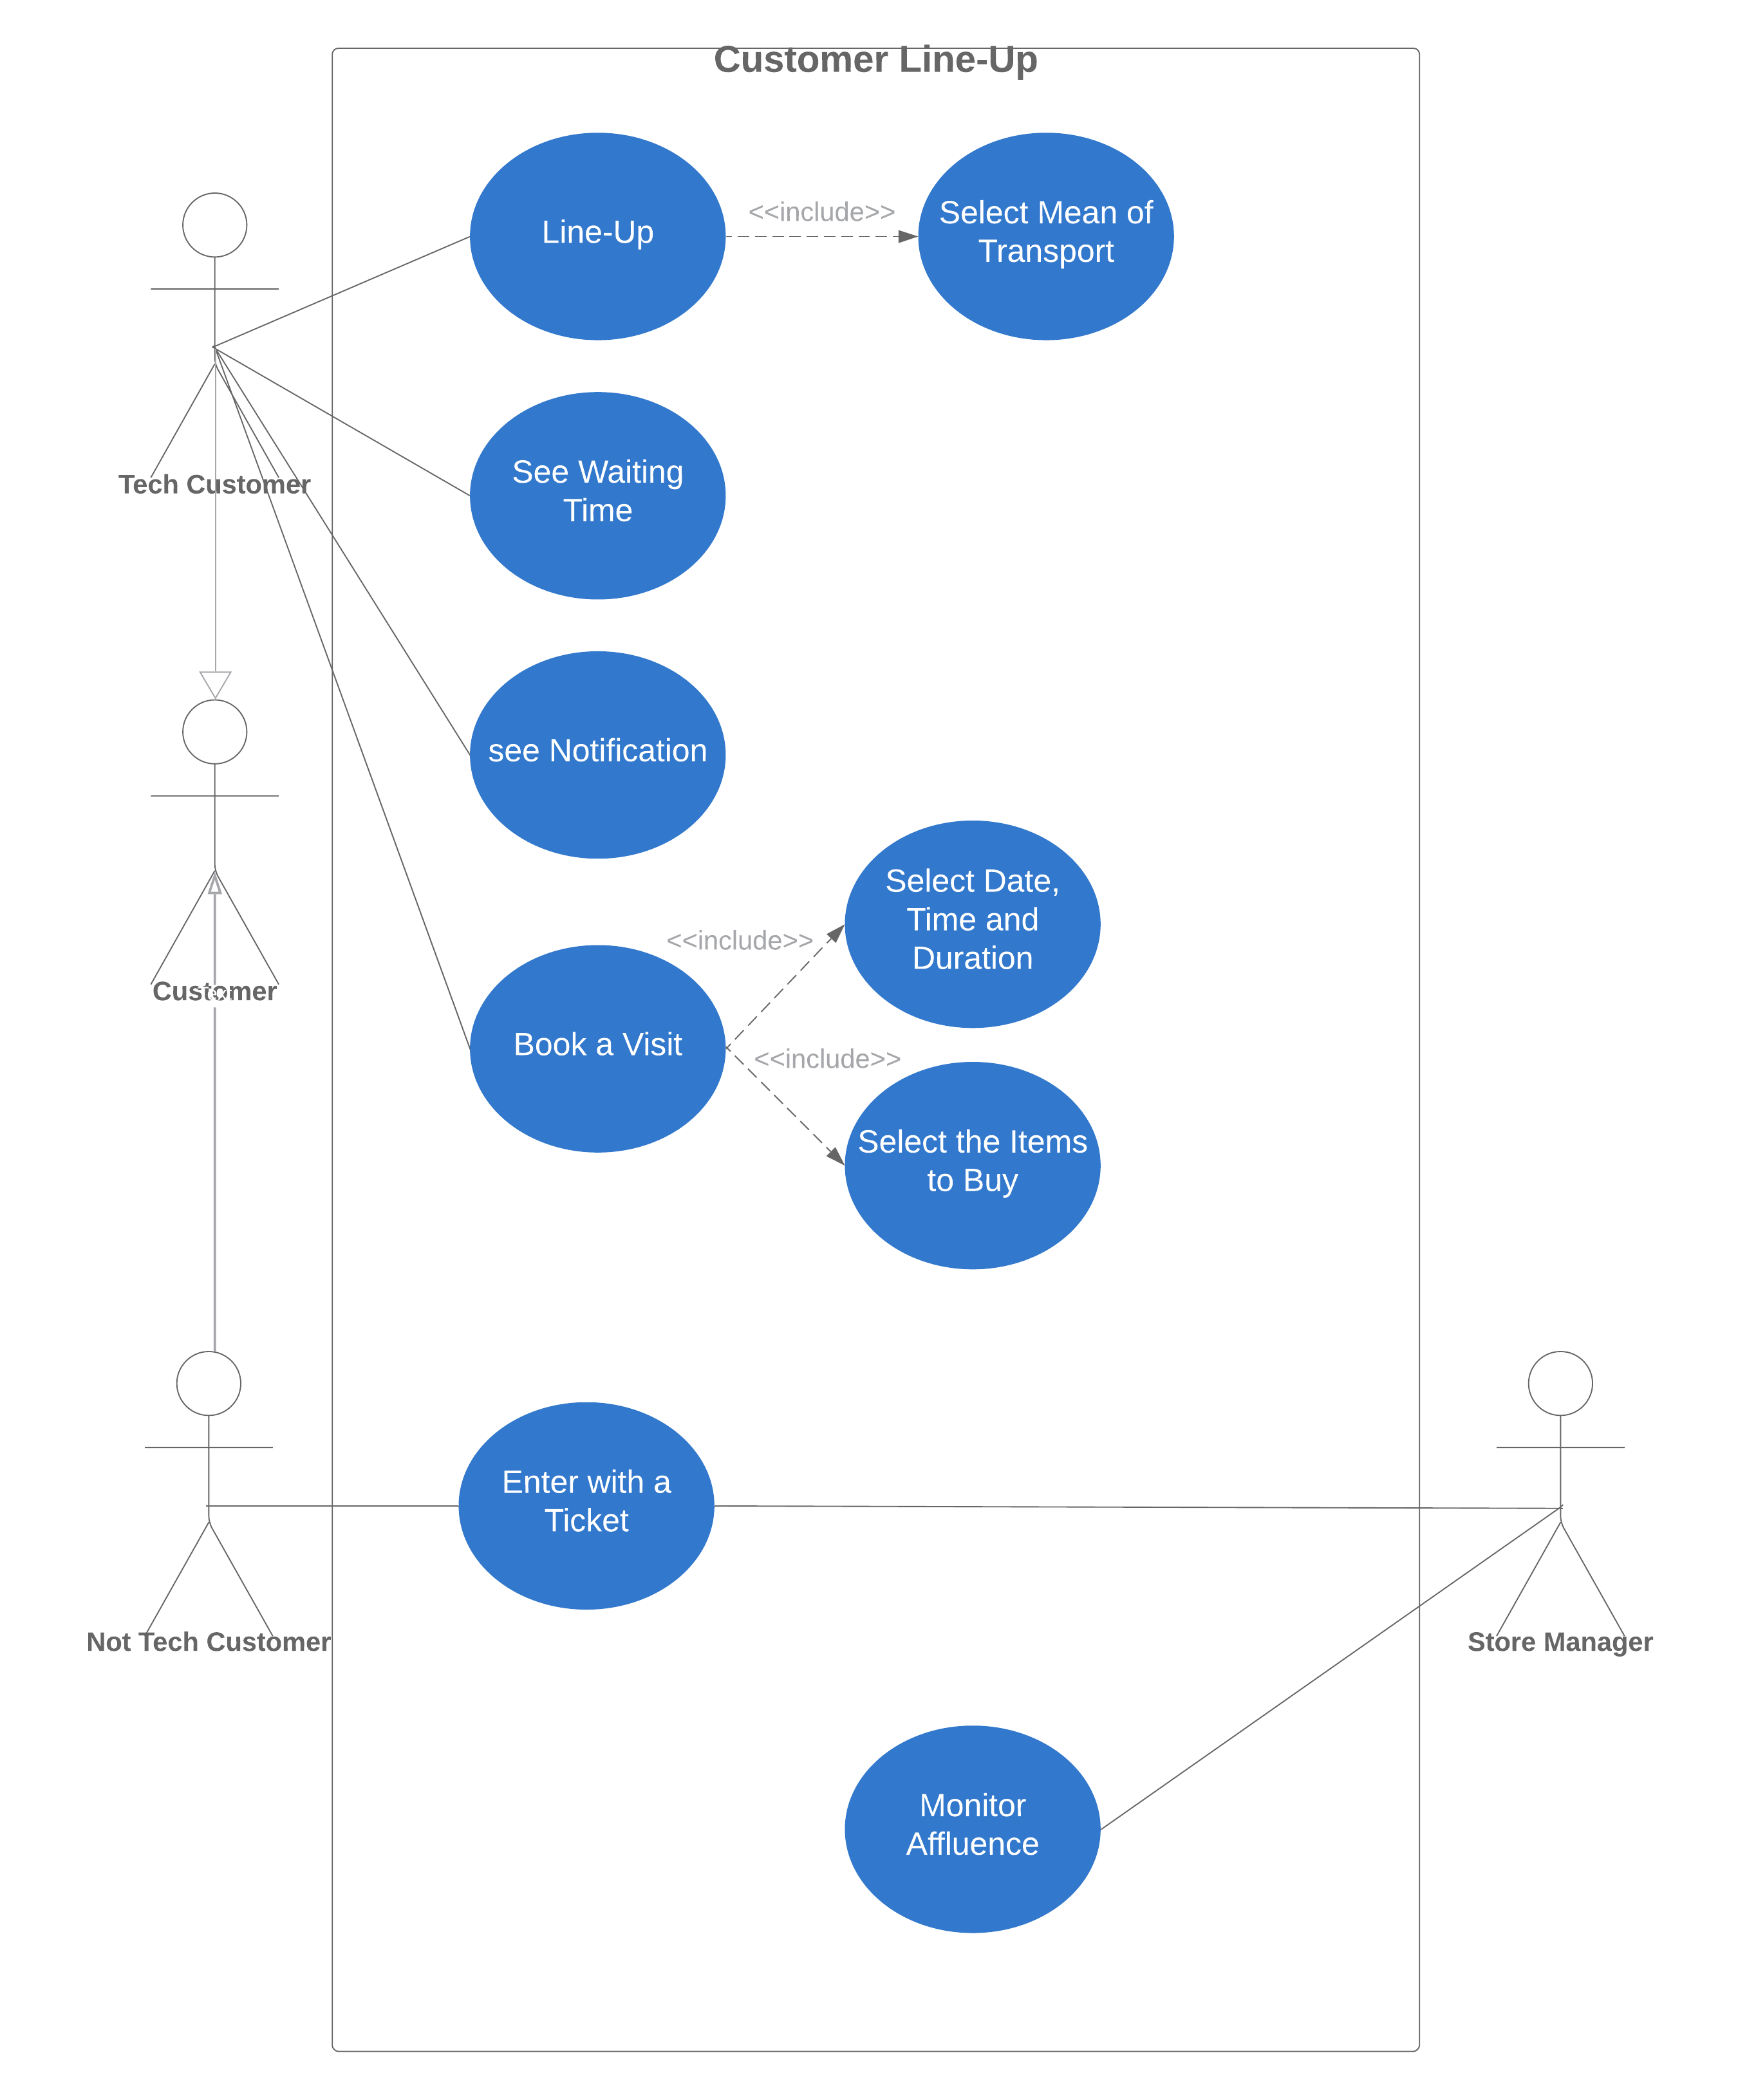
\includegraphics[scale=0.6]{UseCaseDiagram}}
\caption{Use Case Diagram} 
\end{figure}


\textbf{Sequence Diagrams} \\
\textbf{Registration Sequence Diagram} \\
This sequence diagram shows the process of registration made by the Customer: in particular he has to insert the email, username, password and its confirmation. Then, the system verifies the input and if these values are valid then the Customer is successfully registered.
\begin{figure}[H] 
\centerline{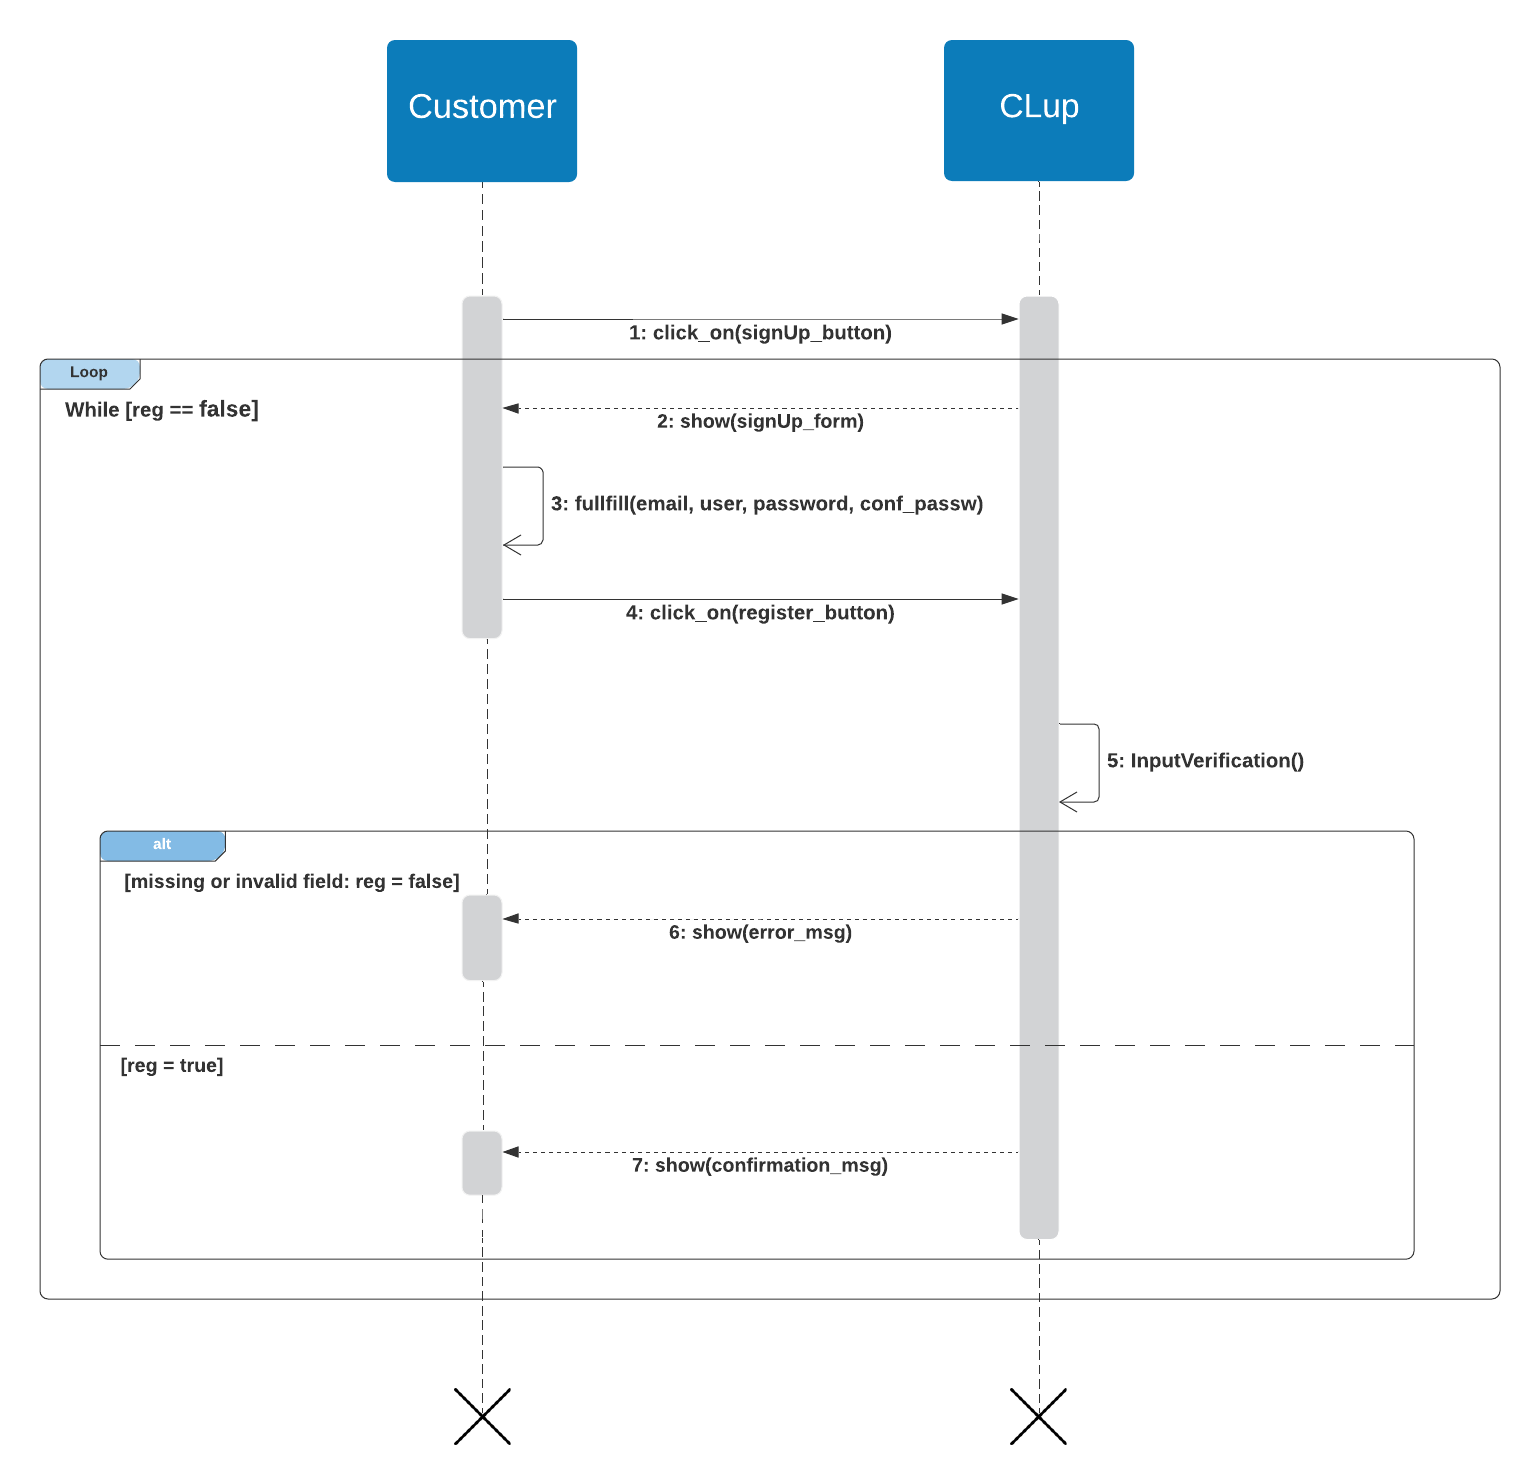
\includegraphics[width=\textwidth]{Registration Sequence Diagram}}
\caption{Registration Sequence Diagram}
\end{figure}



\textbf{Login Sequence Diagram} \\
This sequence diagram shows the process of login made by the Customer: in particular he has to insert his username and password. If the credentials are present in the database, then the Customer can log in.
\begin{figure}[H] 
\centerline{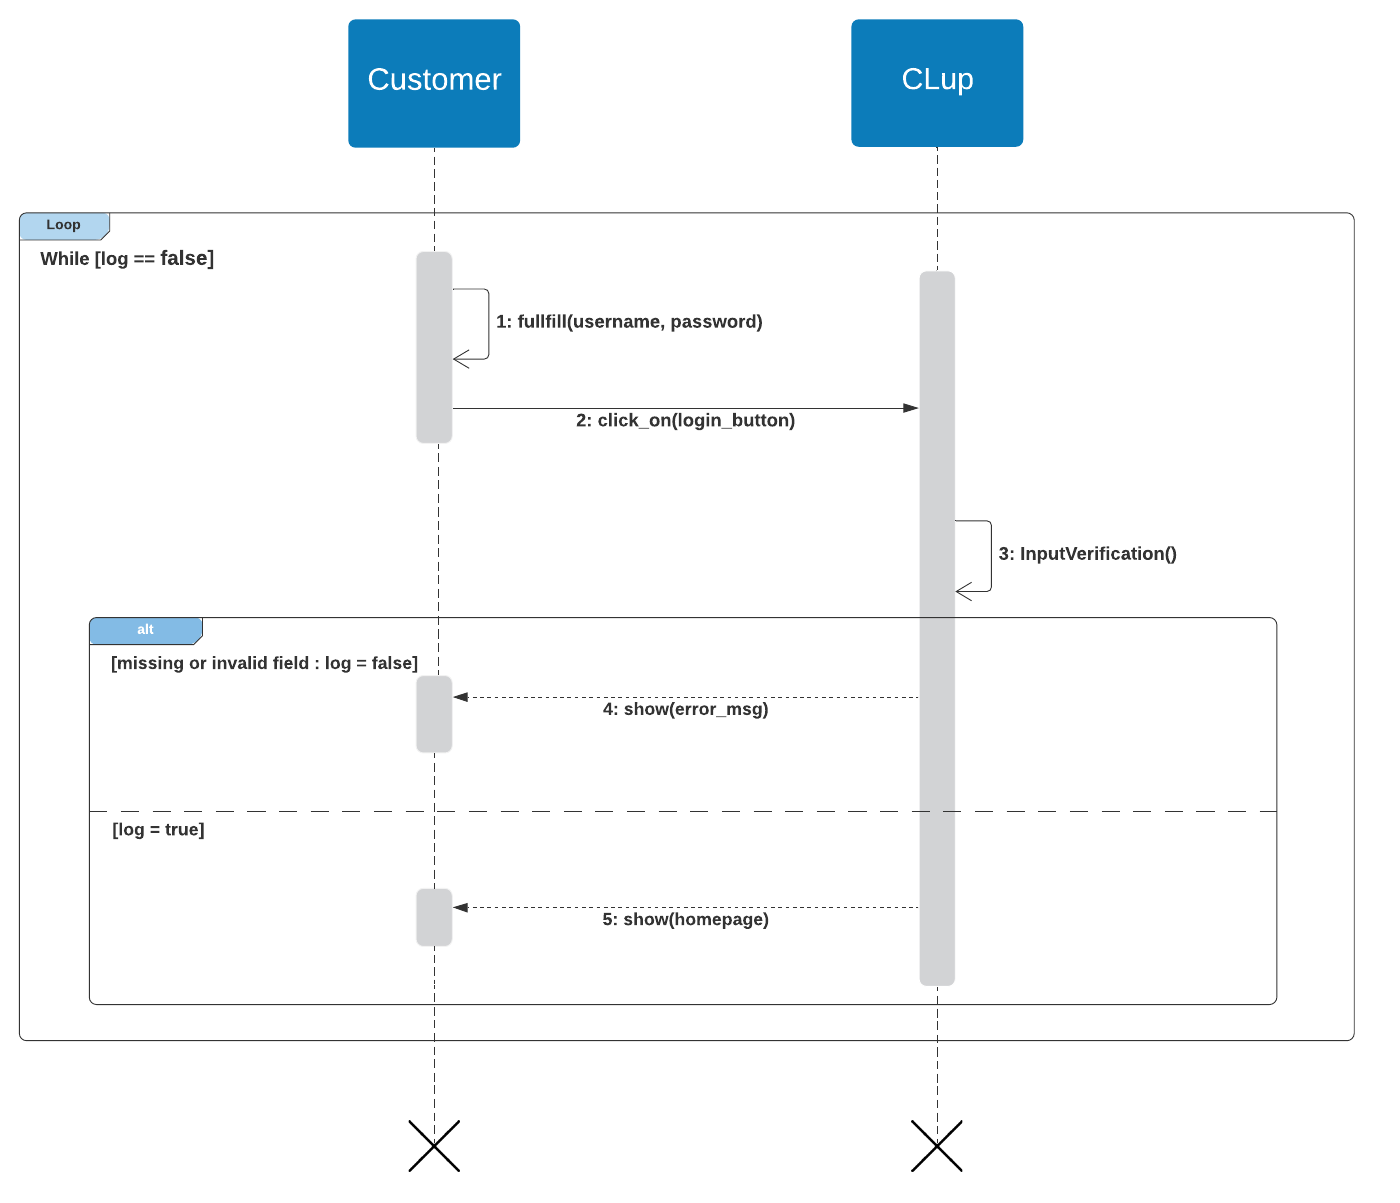
\includegraphics[width=\textwidth]{Login Sequence Diagram}}
\caption{Login Sequence Diagram}
\end{figure}


\textbf{LineUp Sequence Diagram} \\
This sequence diagram shows how the Customer can send a new LineUpRequest: in particular, he has to only select the supermarket, between those available, and his mean of transport. If the parameters are valid, then the LineUpRequest is added to the queue. \\
Notice that it is always possible to send a new LineUpRequest, even if the supermarket is closed: in this case the request will be considered for the first available time slot.
\begin{figure}[H] 
\centerline{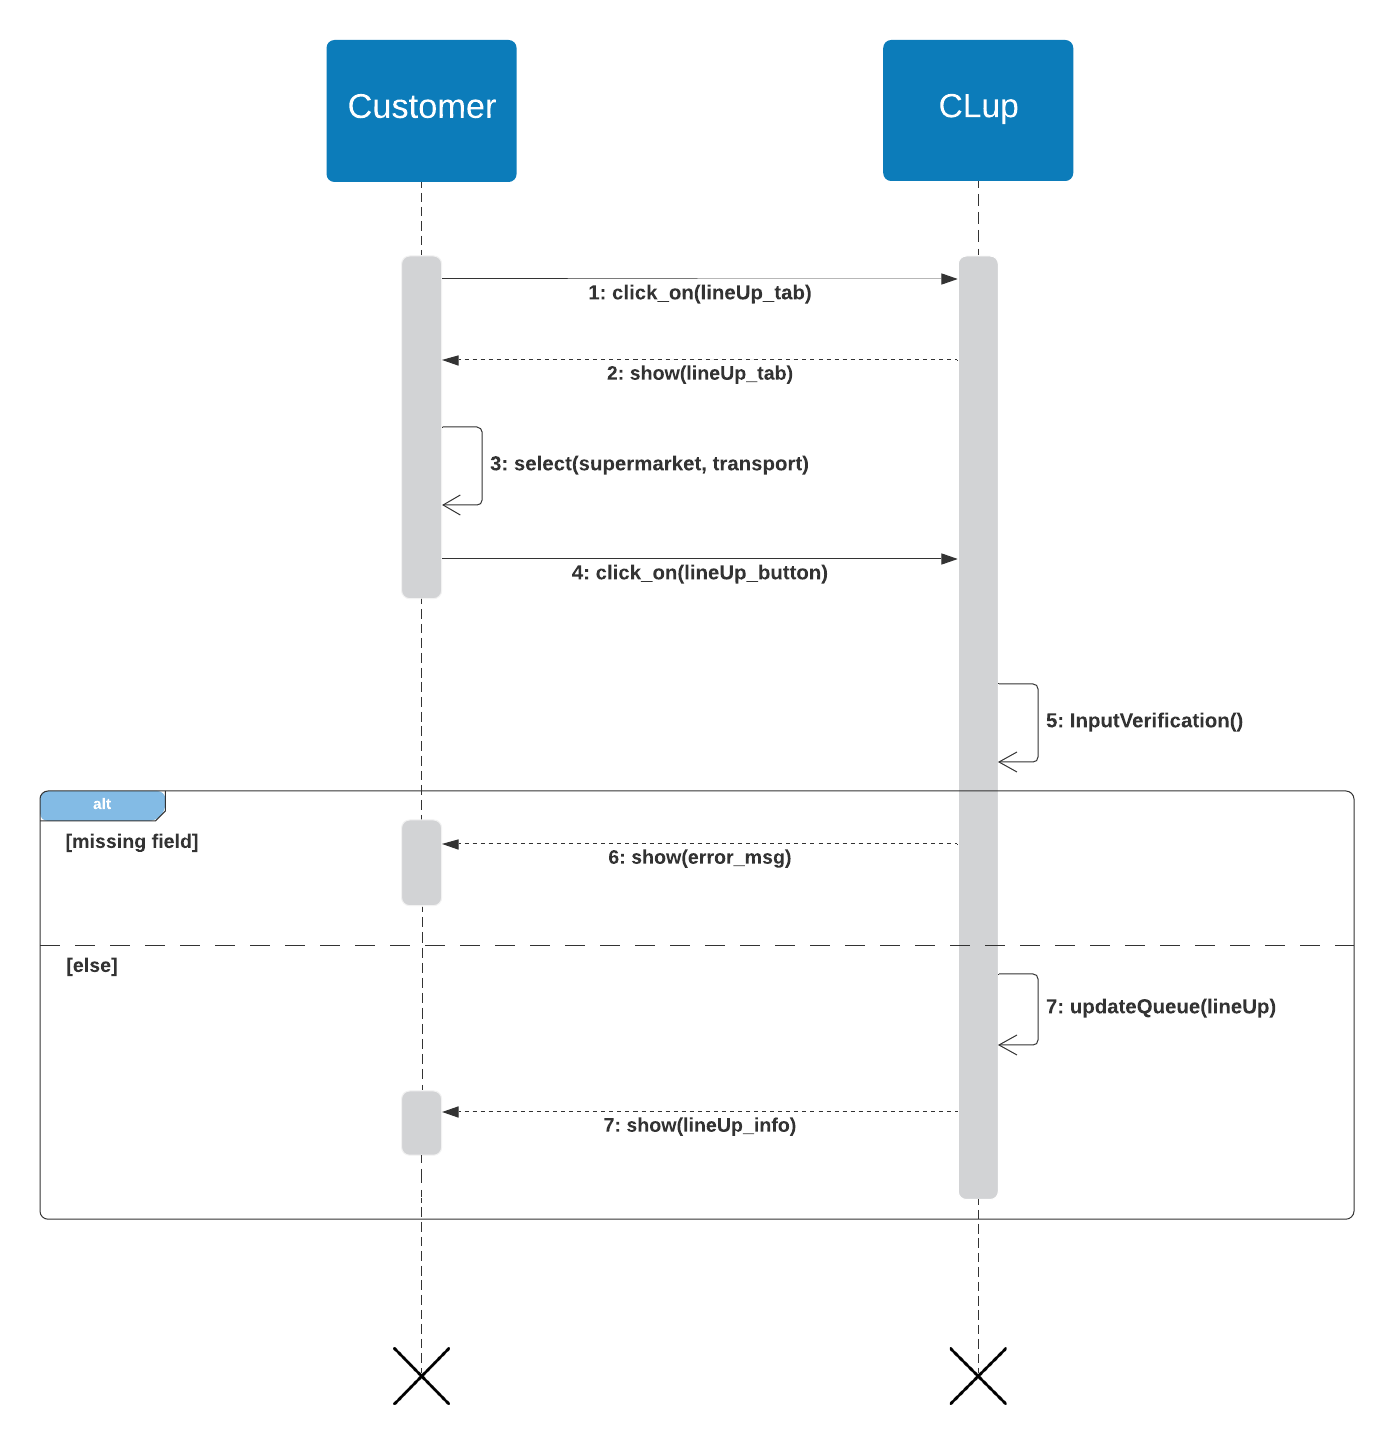
\includegraphics[width=\textwidth]{LineUp Sequence Diagram}}
\caption{Line-Up Sequence Diagram}
\end{figure}



\textbf{Booking Sequence Diagram} \\
This sequence diagram shows how the Customer can send a new BookingRequest: in particular, he has to select the supermarket, between those available, and the day and time of the visit. Moreover, if he is not a longTermCustomer, he is oblied to input also the expectedDuration, while instead the itemsList is optional for all kinds of Customers. Then, the system check all the inputs and if they are valid it saves the BookingRequest. 
\begin{figure}[H] 
\centerline{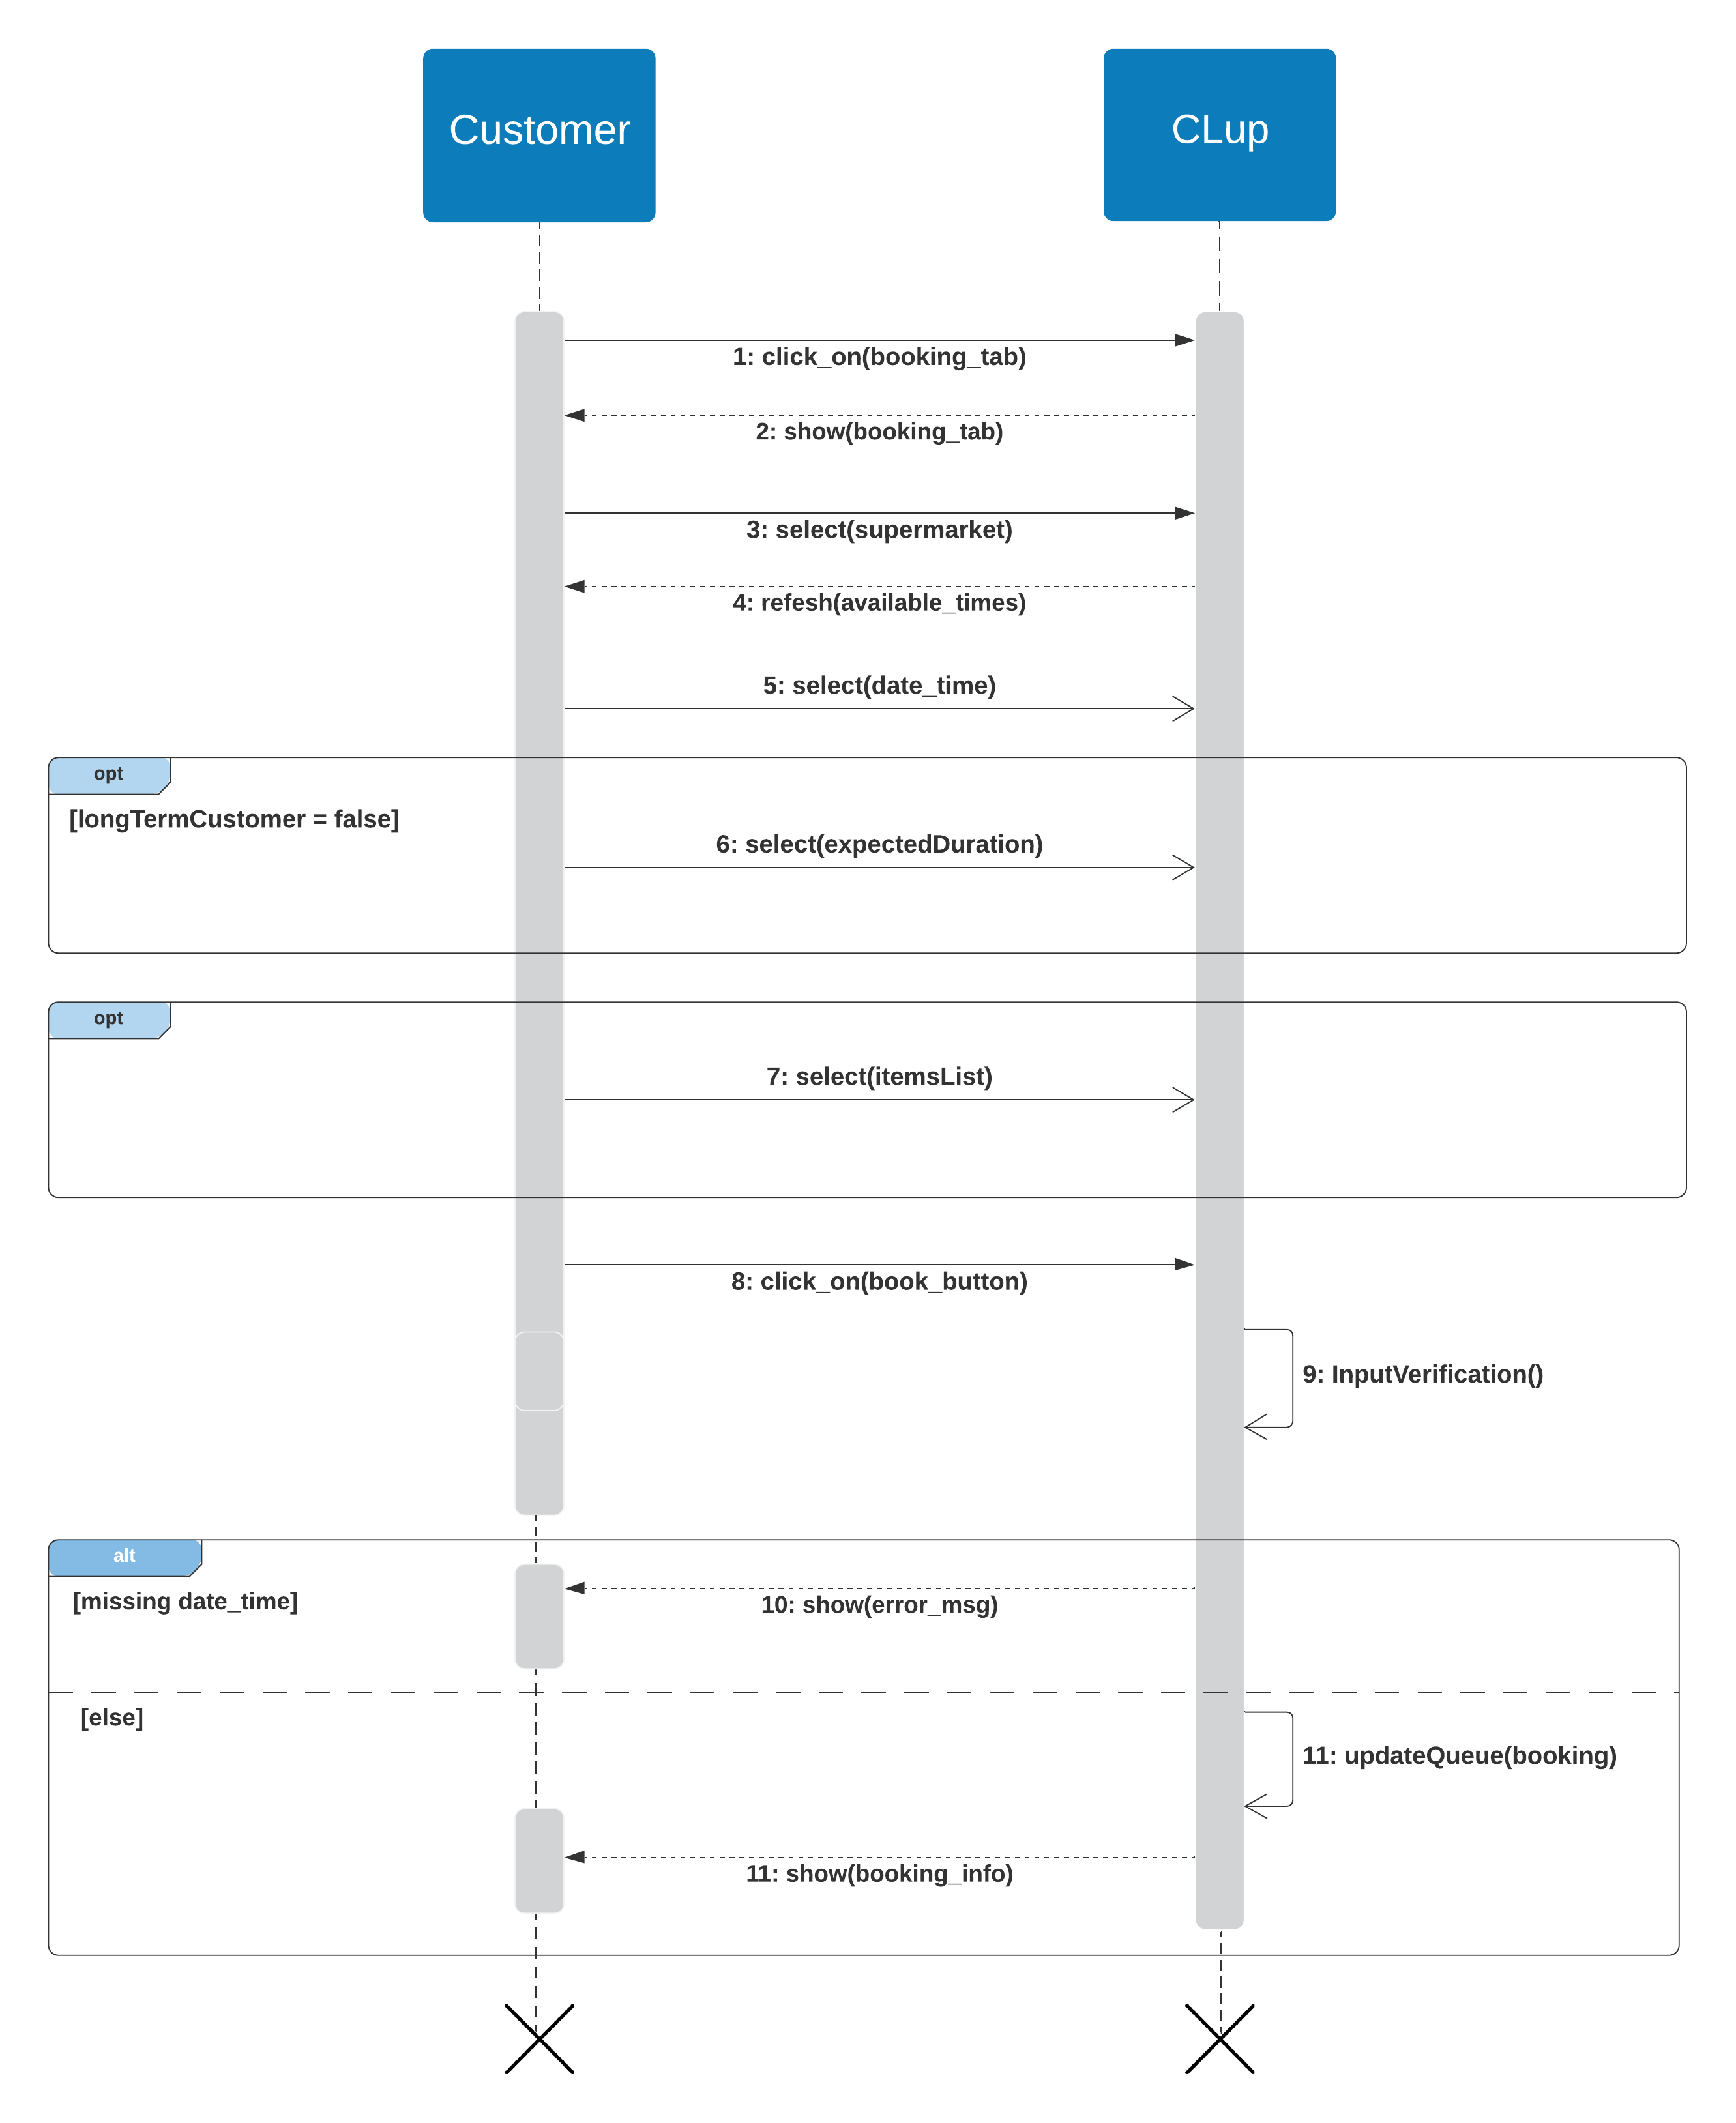
\includegraphics[width=\textwidth]{Booking Sequence Diagram}}
\caption{Booking Sequence Diagram} 
\end{figure}

\textbf{Cancel Booking Sequence Diagram} \\
This sequence diagram shows how the Customer can delete a BookingRequest: in particular, he has only to click on the cancel button, which is shown only if he has an active Booking saved. \\
The analogous canceling procedure can be done for the LineUp.
\begin{figure}[H] 
\centerline{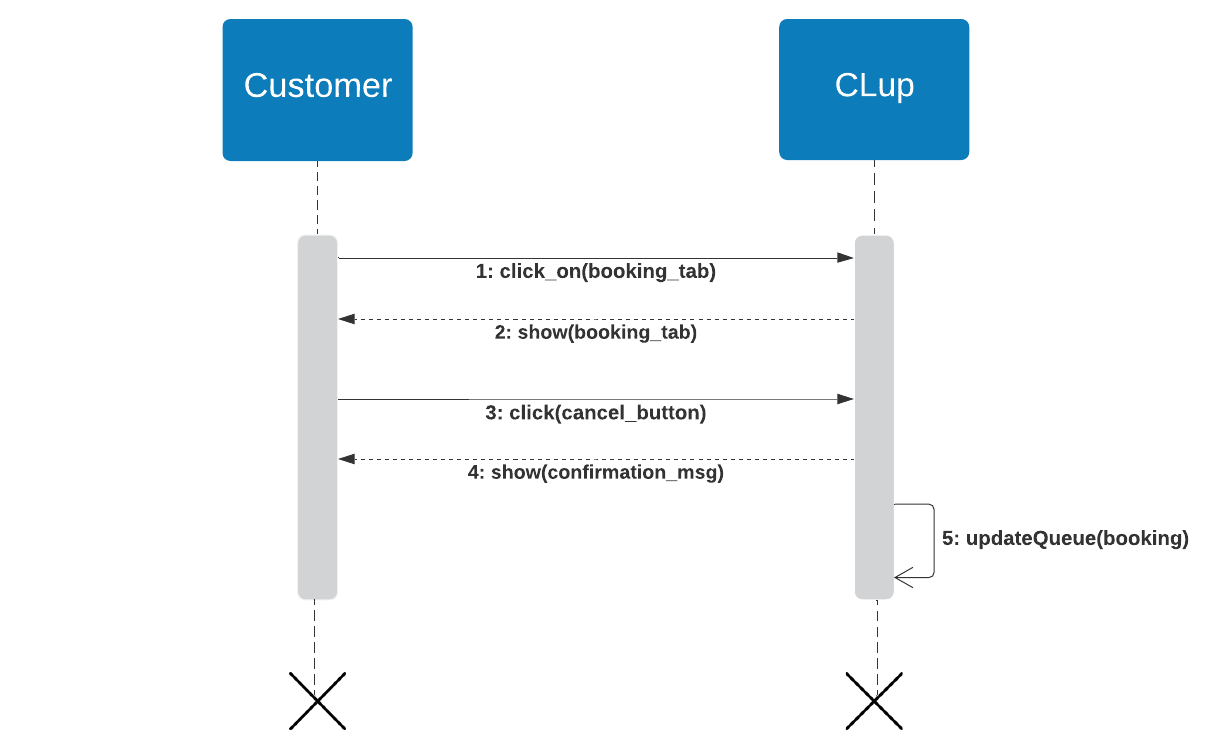
\includegraphics[width=\textwidth]{CancelBooking Sequence Diagram}}
\caption{Cancel Booking Sequence Diagram}
\end{figure}


\textbf{QR-Entrance Sequence Diagram} \\
This sequence diagram shows how the entrance at the supermarket is performed: the Customer has to scan the QRCode and if the system recognized it as valid, then he is allowed to enter.
\begin{figure}[H] 
\centerline{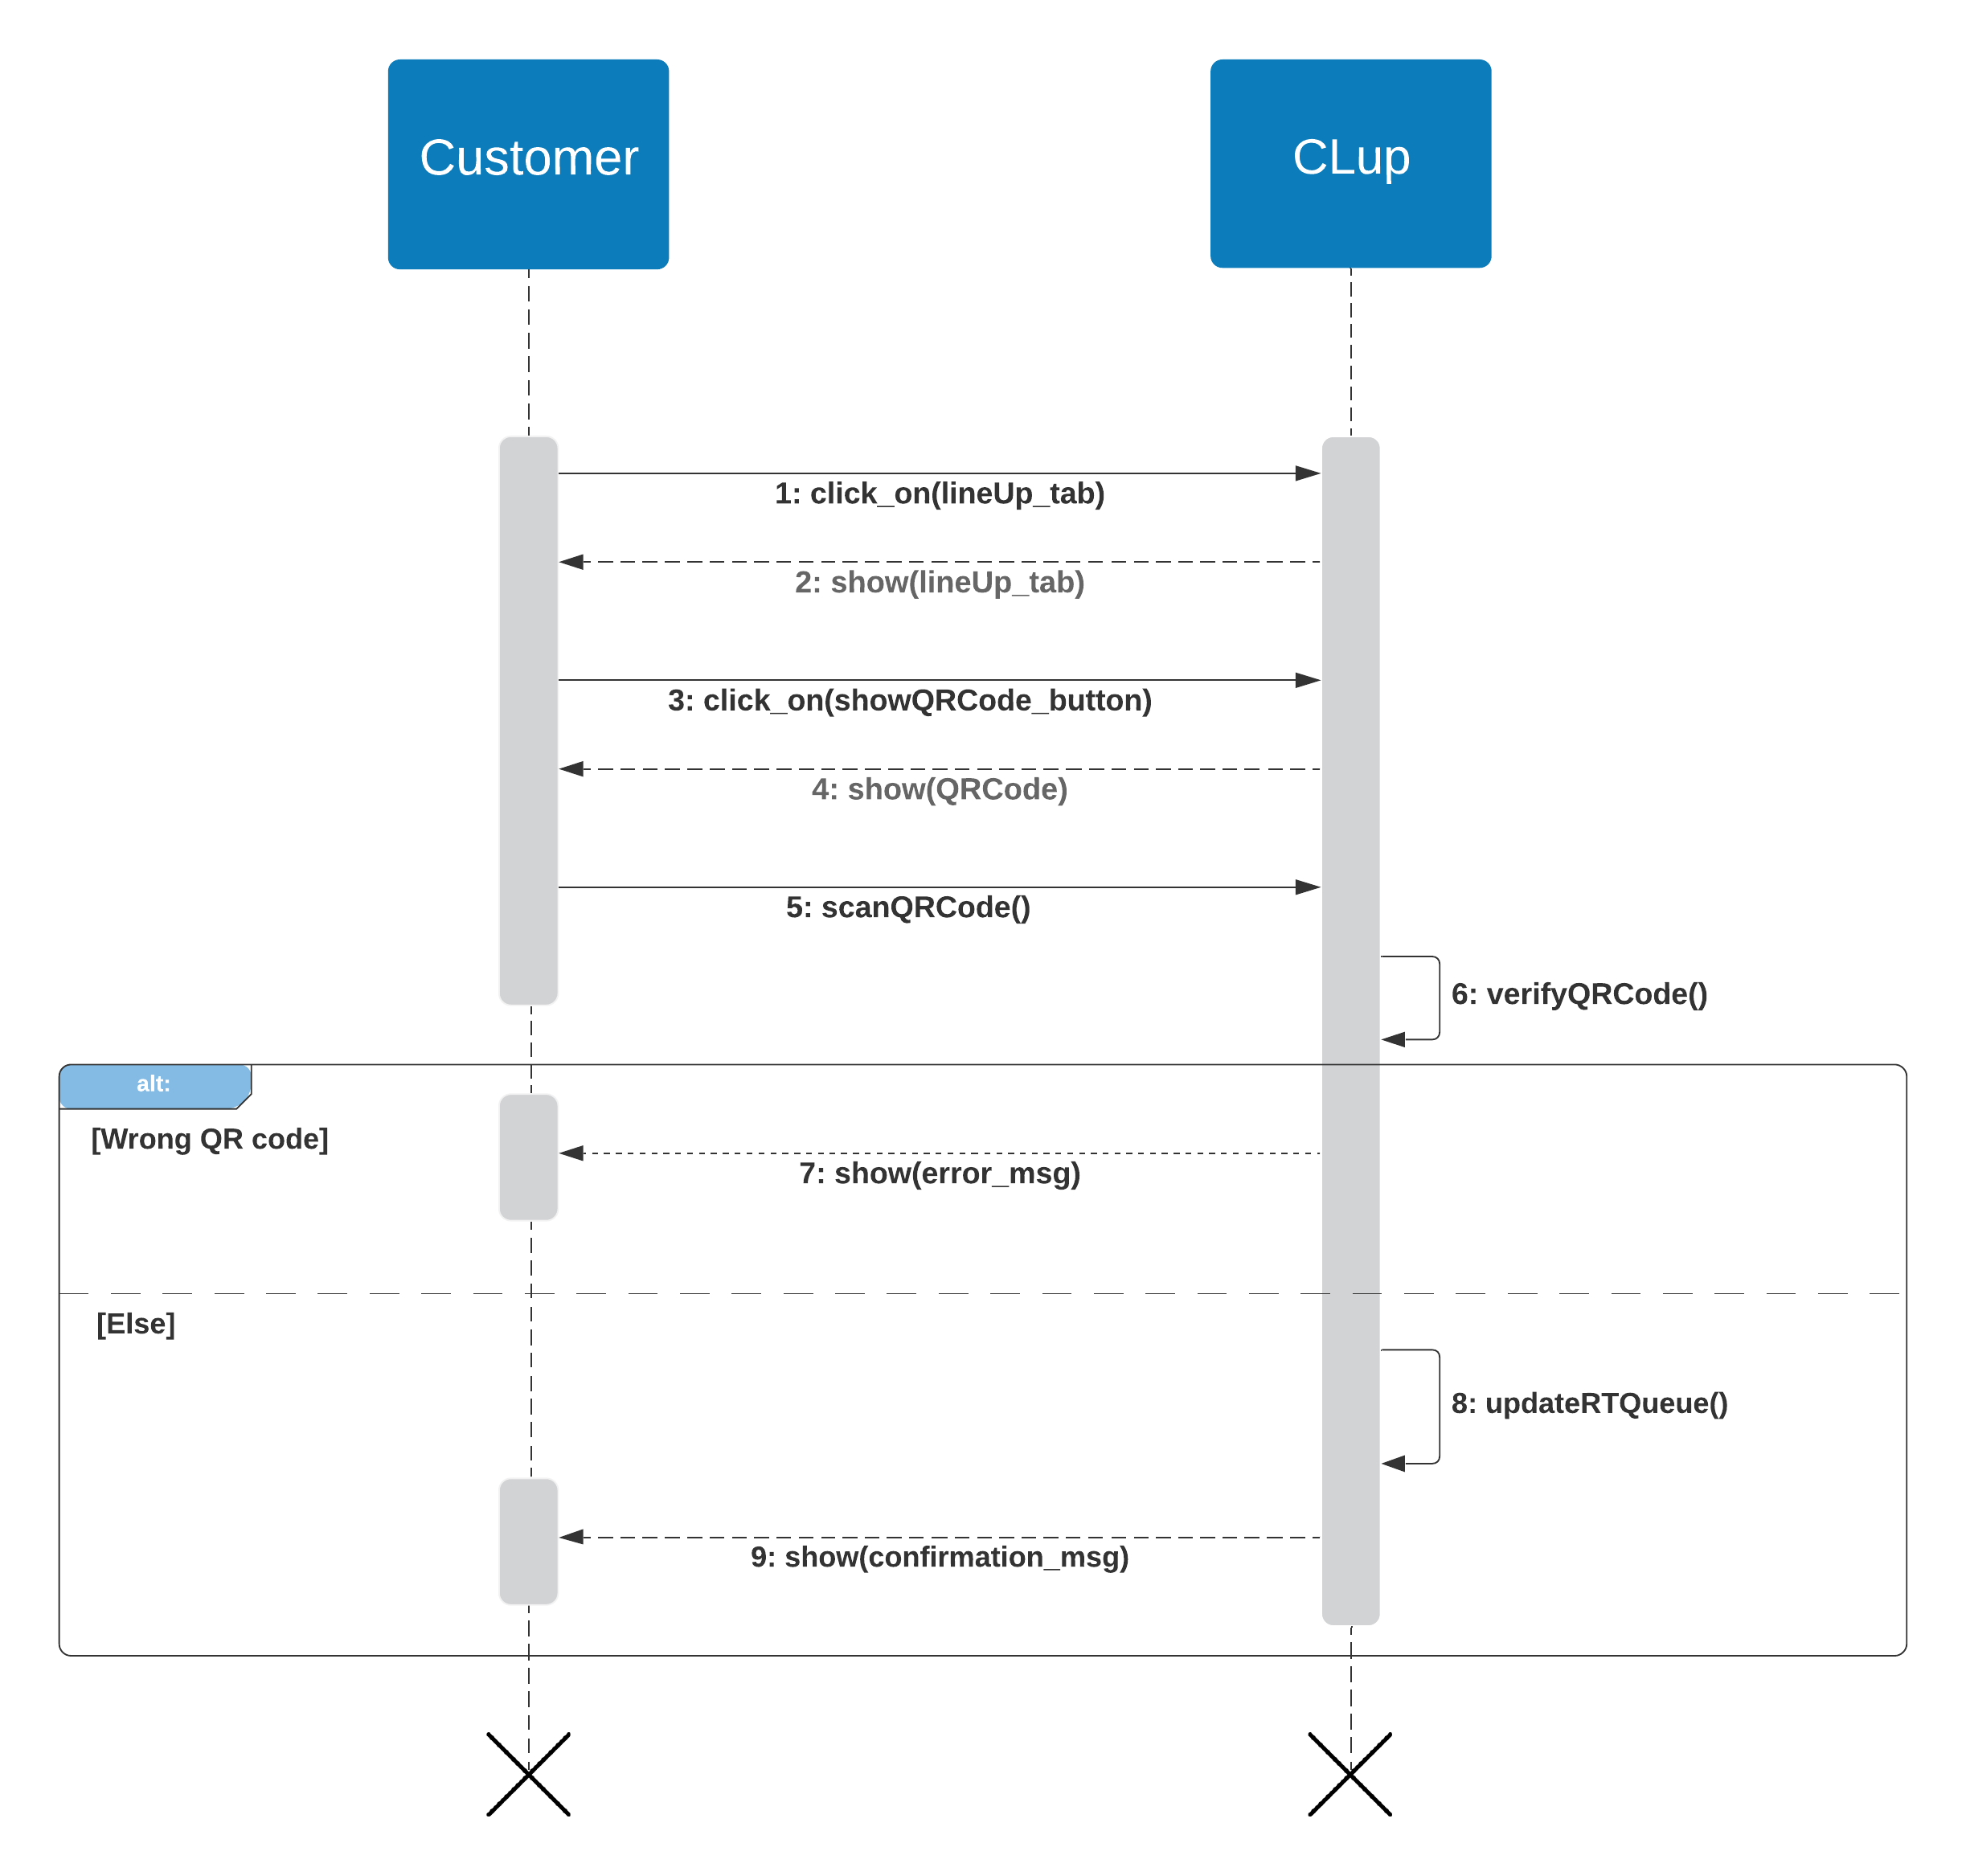
\includegraphics[width=\textwidth]{QR-Entrance Sequence Diagram}}
\caption{QR-Entrance Sequence Diagram}
\end{figure}


\textbf{TicketGeneration Sequence Diagram} \\
This sequence diagram shows the procedure with which the StoreManager can generate a new ticket for a NoTechCustomer. If the supermarket is full, the NoTechCustomer has to wait; otherwise, he can enter and the system updates the affluence data.
\begin{figure}[H] 
\centerline{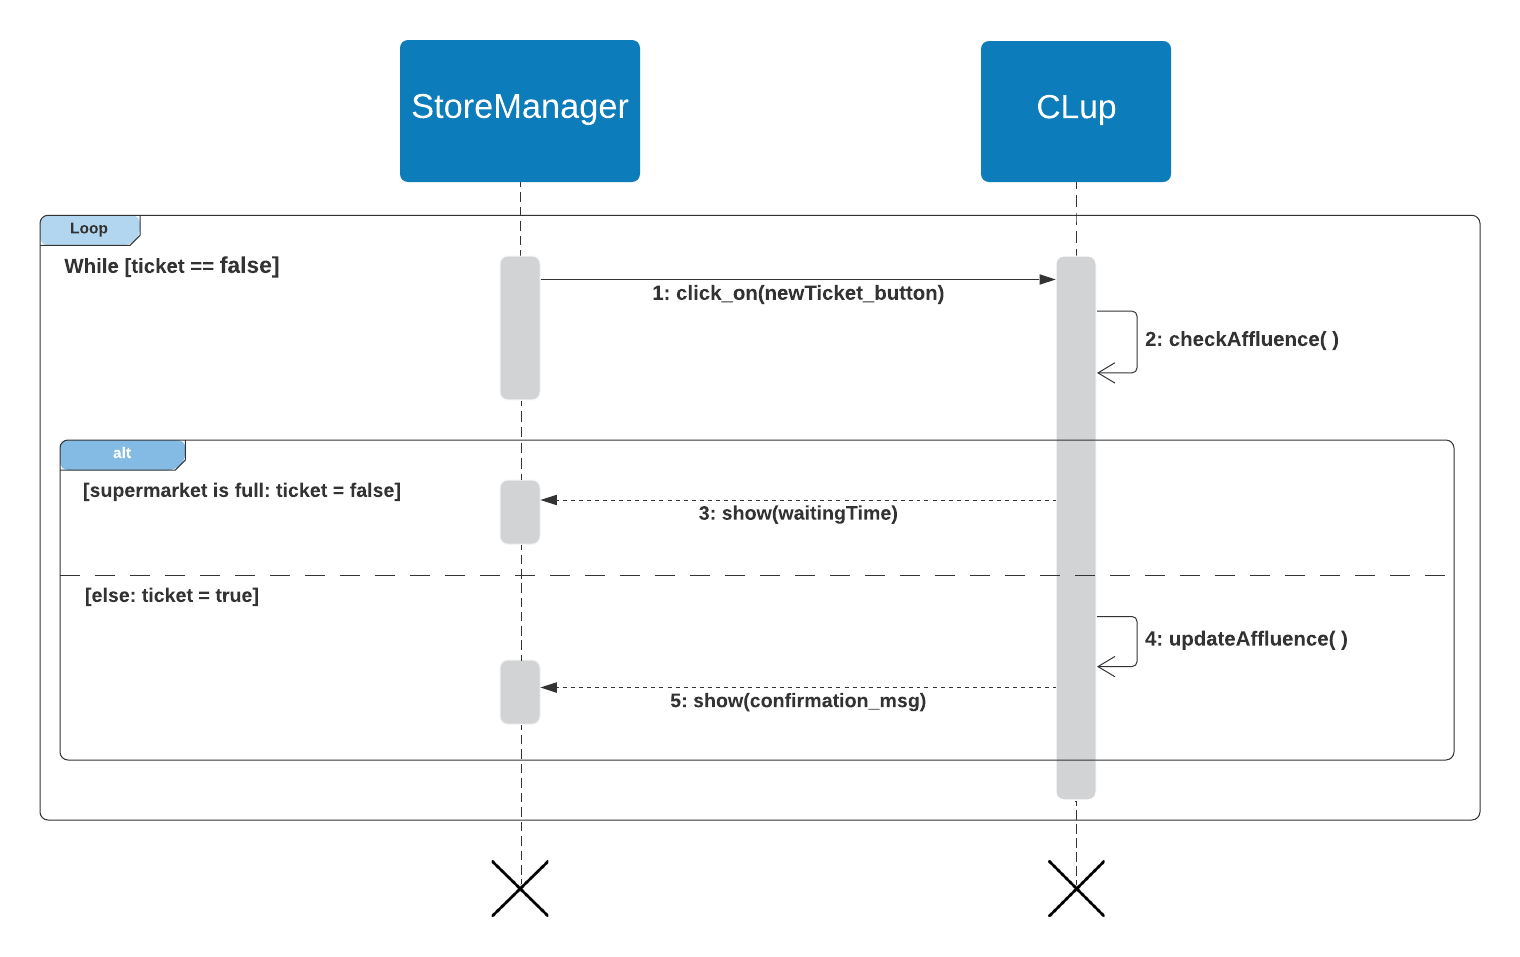
\includegraphics[width=\textwidth]{TicketGeneration Sequence Diagram}}
\caption{Ticket generation Sequence Diagram}
\end{figure}